
\subsubsection{Concept 2}

This concept aims to overcome the problems with the jamming transition encountered by concept 1.
SMA wires are still used for actuation, however rather than a variable stiffness mechanism a mechanical latch will
be used to secure SMA wires around the perch.

This concept can be imagined somewhat like a padlock, roughly illustrated in Fig. \ref{fig:lock}. 
A set of 3 SMA wires will still be used to move between 
home, extended, and latched position. At the end of the wires will be a loop through
which a solenoid, servo, or similar latching mechanism can slide.

\begin{figure}[H]
    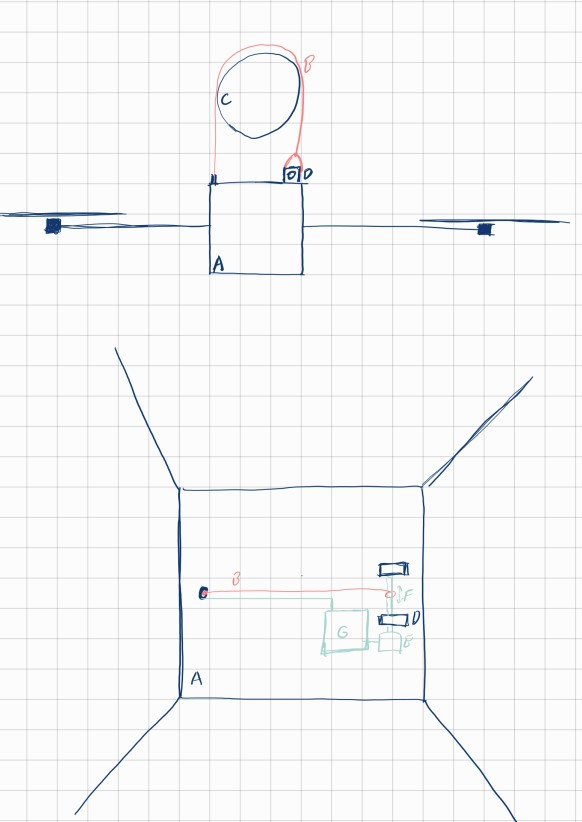
\includegraphics[width=\textwidth]{Lock.jpg}
    \caption{Rough depiction of the lock-like grasping mechanism. Shown is a side profile (top) and a top profile (bottom) 
    of a drone body (A). The SMA wire grasper (B) is shown with a loop at one end, to attach to the latching mechanism (D,F).
    The latch would be driven into place by a small servo (E), controlled from the same unit driving the SMA amplifiers (G).}
    \label{fig:lock}
\end{figure}


\paragraph{Budget}

\begin{table}[ht]
    \centering
    \caption{Estimated budget for the lock design.}
    \label{tab:lock}


    \begin{spreadtab}{{tabular}{|c|c|c|c||c|}}
        \hline
        @Item                       & @Supplier                                                                                                         & @Unit Cost (USD) & @Quantity & @Total Cost (USD) \\
        \hline
        @SMA Wire                   & @\href{https://www.kelloggsresearchlabs.com/product/round-wire/}{Kelloggs Research Labs}                          & 15.99 & 1 & [-1,0] * [-2,0] tag(start) \\
        @Kellogs Shipping           & @-                                                                                                                &  4.99 & 1 & [-1,0] * [-2,0] \\
        @Servo                      & @\href{https://www.digikey.com/en/products/detail/actuonix-motion-devices-inc/L16-50-150-6-R/11689514}{Digikey}   & 90.00 & 1 & [-1,0] * [-2,0] \\
        @Digikey Shipping           & @-                                                                                                                & 14.99 & 1 & [-1,0] * [-2,0] \\
        @Amplifiers                 & @\href{https://www.adafruit.com/product/355}{Adafruit}                                                            &  2.25 & 3 & [-1,0] * [-2,0] \\
        @Arduino                    & @\href{https://www.adafruit.com/product/2378}{Adafruit}                                                           & 11.95 & 1 & [-1,0] * [-2,0] \\
        @FTDI Programmer            & @\href{https://www.adafruit.com/product/70}{Adafruit}                                                             & 19.95 & 1 & [-1,0] * [-2,0] \\
        @Adafruit Shipping          & @-                                                                                                                &  5.08 & 1 & [-1,0] * [-2,0] \\
        @PCB Material               & @\href{https://www.mcmaster.com/8521K873}{McMaster Carr}                                                          & 12.45 & 1 & [-1,0] * [-2,0] \\
        @McMaster Carr Shipping     & @-                                                                                                                & 10.02 & 1 & [-1,0] * [-2,0] \\
        @Mechanical Materials and Fabrication & @-                                                                                                      &     0 & 1 & [-1,0] * [-2,0] tag(pretax)\\
        @Tax                        & @- & sum(cell(start):cell(pretax)) * 0.07 & 1 & [-1,0] * [-2,0] tag(posttax) \\
        @Misc. Spares               & @- & sum(cell(start):cell(posttax)) * 0.2 & 1 & [-1,0] * [-2,0] tag(end) \\
        \hline
        \multicolumn{4}{|c||}{@Total} & sum(cell(start):cell(end)) \\
        \hline
    \end{spreadtab}
\end{table}


\paragraph{Evaluation}

This design has the benefit of being simpler than concept 1, and could possible be made significantly smaller and lighter.

One immediately apparent weakness of this design is that it will not fit to the form of its perch as the coiling, tendril-like 
concept will. This could reduce friction that prevents the drone from swinging on its perch, or sliding back and forth. 
This may possibly be minimized by adding high friction material or spikes to the SMA actuator.
